\subsection{Container to Container Attack}
Containers should not only be isolated from the host, but also from other containers. This allows multiple containers with sensitive data to be run on the same host without them being to access each other's data. In Docker this is not always the case.

\begin{figure}[ht]
    \centering
    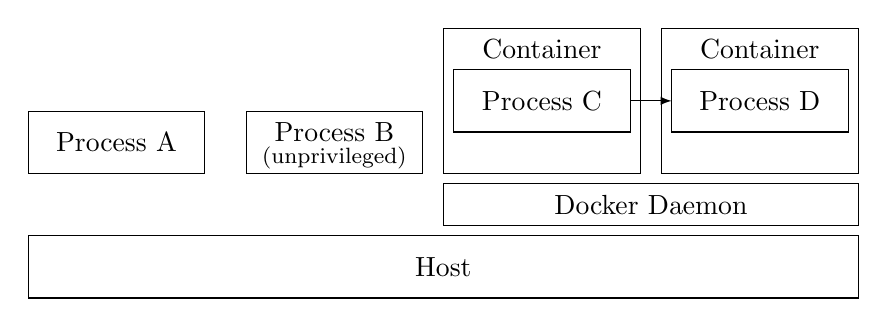
\begin{tikzpicture}[x=0.75pt,y=0.75pt,yscale=-1,xscale=1]
        % Host Rectangle
        \draw (0,100) -- (400,100) -- (400,130) -- (0,130) -- cycle ;
        \draw (200, 115) node {Host};

        %Docker Daemon Rectangle
        \draw (200,75) -- (400,75) -- (400,95) -- (200,95) -- cycle ;
        \draw (300,85) node {Docker Daemon};

        % Process A Rectangle
        \draw (0,40) -- (85,40) -- (85,70) -- (0,70) -- cycle ;
        \draw (42.5,55) node {Process A};

        % Process B Rectangle
        \draw (105,40) -- (190,40) -- (190,70) -- (105,70) -- cycle ;
        \draw (147.5,50) node {Process B};
        \draw (147.5,62.5) node {{\footnotesize (unprivileged)}};

        %Container Process C Rectangle
        \draw (200,0) -- (295,0) -- (295,70) -- (200,70) -- cycle ;
        \draw (247.5,10) node {Container};

        %% Process C Rectangle
        \draw (205,20) -- (290,20) -- (290,50) -- (205,50) -- cycle ;
        \draw (247.5,35) node {Process C};

        %Container Process D Rectangle
        \draw (305,0) -- (400,0) -- (400,70) -- (305,70) -- cycle ;
        \draw (352.5,10) node {Container};

        %% Process D Rectangle
        \draw (310,20) -- (395,20) -- (395,50) -- (310,50) -- cycle ;
        \draw (352.5,35) node {Process D};

        % Line
        \draw [-latex] (290,35) -- (310,35) ;
    \end{tikzpicture}
    \caption{}\label{fig:container-to-container-attack}
    \medskip
    \small
    A process (Process C) running inside a container, accessing data in another container (process D).
\end{figure}

By default all Docker containers are added to the same bridge network. This means that (by default) all Docker containers can reach each other over the network. This differs from the isolation Docker uses for other namespaces. In the other namespaces, Docker (by default) isolates containers from the host and other containers. This design decision can lead to very dangerous situations, because developers may believe that Docker containers are completely isolated from each other (including the network).
